% Báo cáo môn Học máy với dữ liệu đồ thị: hai bài báo MMKGC (HFR-MKGC và MDBGF).
% Biên dịch: xelatex mmkgc-report && bibtex mmkgc-report && xelatex mmkgc-report && xelatex mmkgc-report
% Hoặc chạy build.sh trong cùng thư mục. File nộp: 25C11050-25C15003.pdf
\documentclass[conference,a4paper]{IEEEtran}

\usepackage{fontspec}
\setmainfont{Times New Roman}
\usepackage{polyglossia}
\setdefaultlanguage{vietnamese}
\usepackage{amsmath,amssymb}
\usepackage{graphicx}
\usepackage{booktabs}
\usepackage{multirow}
\usepackage{xcolor}
\usepackage{tikz}
\usetikzlibrary{arrows.meta,positioning,calc,fit,backgrounds}
\usepackage{pgfplots}
\pgfplotsset{compat=1.18}
\usepackage{enumitem}
\setlist{nosep,leftmargin=*}
\usepackage{url}
\usepackage[hidelinks]{hyperref}
\usepackage{etoolbox}
\gappto\captionsvietnamese{\renewcommand{\refname}{Tài liệu tham khảo}}
\renewcommand{\IEEEkeywordsname}{Từ khoá}

\graphicspath{{figures/}}

% Màu dùng chung cho hình tự vẽ
\definecolor{cS}{HTML}{2A6F97}   % cấu trúc
\definecolor{cI}{HTML}{C8553D}   % ảnh
\definecolor{cT}{HTML}{2A9D8F}   % văn bản
\definecolor{cR}{HTML}{E9C46A}   % quan hệ
\definecolor{cG}{HTML}{8E6CAD}   % cổng / MLLM
\definecolor{cGray}{HTML}{5C6570}

\newcommand{\Hj}{\mathbf{H}_{\mathrm{joint}}}
\newcommand{\Tj}{\mathbf{T}_{\mathrm{joint}}}
\newcommand{\Tm}{\mathbf{T}_{\mathrm{MLLM}}}
\newcommand{\Tt}{\tilde{\mathbf{T}}}
\renewcommand{\Re}{\operatorname{Re}}
\renewcommand{\Im}{\operatorname{Im}}
\newcommand{\todo}[1]{\textcolor{red}{[#1]}}

\begin{document}

\title{Hoàn thiện đồ thị tri thức đa phương thức:\\
tìm hiểu hai công trình HFR-MKGC và MDBGF}

\author{
\IEEEauthorblockN{Nguyễn Đình Lộc (25C11050) \qquad Ngô Trương Minh Đạt (25C15003)}
\IEEEauthorblockA{Khoa Công nghệ Thông tin, Trường Đại học Khoa học Tự nhiên, ĐHQG-HCM\\
Học phần: Học máy với dữ liệu đồ thị \quad Giảng viên: TS. Lê Ngọc Thành}
}

\maketitle

\begin{abstract}
Báo cáo này trình bày cách hiểu của nhóm về hai công trình gần đây trong bài toán hoàn thiện đồ thị tri thức đa phương thức (Multi-modal Knowledge Graph Completion, MMKGC). Phần thứ nhất phân tích HFR-MKGC (AAAI 2026), một khung kết hợp ba ý tưởng trên nền hàm điểm RotatE: trộn ba mô thức của thực thể với trọng số phụ thuộc quan hệ đang xét, đưa dự đoán của một mô hình ngôn ngữ lớn đa phương thức vào hàm điểm thông qua một cổng học được, và huấn luyện đối kháng với mẫu âm sinh bằng cách bóp méo đặc trưng ảnh và văn bản. Nhóm diễn giải lại từng mô-đun bằng một ví dụ chạy tay xuyên suốt, tổng hợp kết quả thực nghiệm trên ba bộ dữ liệu chuẩn và chỉ ra các điểm chưa thuyết phục của bài báo. Phần thứ hai phân tích MDBGF (Findings of ACL 2026), tiếp cận bài toán theo hướng ngược lại: chủ động làm rụng mô thức khi huấn luyện và hợp nhất hai chiều để mô hình bền vững khi thiếu dữ liệu. Phần cuối đối chiếu hai hướng tiếp cận và rút ra bài học chung.
\end{abstract}

\begin{IEEEkeywords}
đồ thị tri thức, hoàn thiện đồ thị tri thức, học biểu diễn đa phương thức, mô hình ngôn ngữ lớn đa phương thức, huấn luyện đối kháng
\end{IEEEkeywords}

% =====================================================================
\section{Giới thiệu chung}
\label{sec:intro}

\subsection{Bài toán}

Một đồ thị tri thức (Knowledge Graph, KG) lưu sự thật dưới dạng bộ ba $(h, r, t)$: thực thể đầu $h$, quan hệ $r$ và thực thể đuôi $t$. Ví dụ (Gwen Stefani, voice type, Mezzo-soprano). KG xây dựng tự động hay bán tự động luôn thiếu cạnh, nên bài toán hoàn thiện đồ thị tri thức (Knowledge Graph Completion, KGC) đặt câu hỏi: cho $(h, r, ?)$ hoặc $(?, r, t)$, thực thể nào điền vào chỗ trống là hợp lý nhất. Đây là bài toán dự đoán liên kết, không phải sinh thực thể mới: đáp án luôn là một node đã có trong đồ thị.

Trong KG đa phương thức (Multi-modal KG, MMKG), mỗi thực thể ngoài vị trí trong đồ thị còn có một đoạn mô tả văn bản và một hoặc nhiều ảnh. MMKGC là KGC trên dữ liệu đó. Câu hỏi trung tâm của cả hai bài báo trong báo cáo này là: dùng văn bản và ảnh thế nào để chúng giúp dự đoán thay vì gây nhiễu, nhất là khi một phần thực thể thiếu ảnh hoặc thiếu mô tả.

Theo thuật ngữ của môn học, hai bài báo đều thuộc nhóm nhúng đồ thị tri thức (Knowledge Graph Embedding, KGE): mỗi thực thể và mỗi quan hệ là một hàng trong bảng tham số, không có bước truyền tin giữa các node như mạng nơ-ron đồ thị (GNN). Cấu trúc đồ thị đi vào mô hình qua hàm mất mát: mỗi cạnh trong tập huấn luyện là một ràng buộc buộc vector của $h$, $r$, $t$ phải khớp nhau theo một hàm điểm. Vì không có phép gom láng giềng, câu hỏi về bất biến hoán vị không phát sinh.

\subsection{Cách đánh giá chung}

Với mỗi bộ ba kiểm thử, mô hình che một đầu, chấm điểm toàn bộ thực thể làm ứng viên và xếp hạng. Đáp án đúng đứng hạng càng cao càng tốt. Hai độ đo được dùng: MRR (trung bình nghịch đảo hạng) và Hits@$K$ (tỉ lệ đáp án đúng nằm trong $K$ hạng đầu). Cả hai bài đều dùng thiết lập lọc (filtered): các đáp án đúng khác đã có trong KG bị loại khỏi danh sách xếp hạng để không bị phạt oan. Cả hai chiều $(h,r,?)$ và $(?,r,t)$ đều được hỏi.

Ba bộ dữ liệu chuẩn xuất hiện trong cả hai bài: MKG-W và MKG-Y~\cite{mkgwy} (trích từ Wikidata và YAGO), DB15K~\cite{mmkg} (trích từ DBpedia). Thống kê ở Bảng~\ref{tab:datasets}; hai cột cuối là tỉ lệ thực thể có ảnh và có văn bản, nhóm tự tính từ số liệu gốc. Điểm đáng chú ý là DB15K thiếu văn bản ở gần 30\% thực thể, còn MKG-Y chỉ có 28 quan hệ nên cấu trúc đã rất giàu thông tin.

\begin{table}[t]
\centering
\caption{Ba bộ dữ liệu MMKGC dùng trong cả hai bài báo. Số liệu theo~\cite{hfrmkgc}; hai cột cuối do nhóm tính.}
\label{tab:datasets}
\footnotesize
\setlength{\tabcolsep}{3pt}
\begin{tabular}{l rrrrr cc}
\toprule
Bộ dữ liệu & \#Ent & \#Rel & \#Train & \#Valid & \#Test & Có ảnh & Có văn bản\\
\midrule
MKG-W & 15000 & 169 & 34196 & 4276 & 4274 & 96{,}4\% & 94{,}2\%\\
MKG-Y & 15000 & 28  & 21310 & 2665 & 2663 & 95{,}0\% & 82{,}0\%\\
DB15K & 12842 & 279 & 79222 & 9902 & 9904 & 99{,}8\% & 70{,}7\%\\
\bottomrule
\end{tabular}
\end{table}

\subsection{Cấu trúc báo cáo}

Phần~\ref{sec:hfr} dành cho HFR-MKGC~\cite{hfrmkgc}, bài nhóm đã trình bày seminar. Phần~\ref{sec:mdbgf} dành cho MDBGF~\cite{mdbgf}. Phần~\ref{sec:compare} đối chiếu hai bài và kết luận. Mọi số liệu thực nghiệm được lấy từ bài báo gốc và ghi rõ nguồn; nhóm không chạy lại thực nghiệm của HFR-MKGC vì tác giả không công khai mã nguồn.

% =====================================================================
\section{Phần A: HFR-MKGC}
\label{sec:hfr}

\subsection{Động lực và ý tưởng chính}
\label{sec:hfr-motivation}

Để thấy vì sao cần đa mô thức, hãy lấy truy vấn xuyên suốt của báo cáo: (Gwen Stefani, voice type, ?). Trong MKG-W, thực thể này chỉ có một cạnh huấn luyện là field of work $\to$ music. Nếu chỉ nhìn cấu trúc, gần như không có căn cứ để chọn giữa Mezzo-soprano, Soprano hay hàng nghìn node khác. Đoạn mô tả có chữ ``singer'' và ảnh chân dung mới là thứ gợi ý rằng đáp án phải là một loại giọng hát.

Từ góc nhìn của nhóm, bài báo chỉ ra hai điểm yếu của các phương pháp trước và đề xuất một cách sửa cho mỗi điểm:

\begin{enumerate}
\item \textbf{Trọng số trộn mô thức không phụ thuộc câu hỏi.} Các mô hình như RSME~\cite{rsme} hay NativE~\cite{native} trộn cấu trúc, ảnh, văn bản bằng cổng hoặc chú ý, nhưng tỉ lệ trộn của một thực thể là cố định hoặc chỉ phụ thuộc chính thực thể đó. Với Gwen Stefani, ảnh hữu ích khi hỏi giới tính nhưng vô ích khi hỏi loại giọng; một bộ trọng số không thể đúng cho cả hai câu hỏi. HFR-MKGC đưa vector quan hệ vào công thức tính trọng số, nên cùng một thực thể có tỉ lệ trộn khác nhau tuỳ quan hệ đang xét.
\item \textbf{Mô hình ngôn ngữ lớn (LLM) được dùng thô.} Các phương pháp dựa trên LLM biến đồ thị thành prompt rồi để LLM trả lời, nhưng LLM không biết ranh giới tập thực thể, hay bịa tên, và không chấm điểm được toàn bộ ứng viên. Bảng~\ref{tab:main} xác nhận điều đó: LLaVA chạy một mình chỉ đạt Hits@10 bằng 26{,}42\% trên MKG-W và 3{,}58\% trên MKG-Y. HFR-MKGC không cho LLM làm bộ chấm điểm mà coi câu trả lời của nó là một gợi ý, đưa vào hàm điểm RotatE qua một cổng có thể học mức tin cậy.
\end{enumerate}

Ý thứ ba của bài là về huấn luyện: mẫu âm thay ngẫu nhiên thực thể đuôi quá dễ phân biệt, nên tác giả sinh thêm mẫu âm ``khó'' bằng cách giữ nguyên thực thể nhưng bóp méo đặc trưng ảnh và văn bản, rồi huấn luyện theo kiểu đối kháng.

Tên bài gói ba ý này thành ba mô-đun: RHF (Relation-guided Hierarchical Fusion, hợp nhất phân cấp có dẫn hướng bởi quan hệ), MER (MLLM-Enhanced Reasoning, suy luận tăng cường bằng MLLM) và MNO (Multi-modal Noise Optimization, tối ưu nhiễu đa mô thức). Hình~\ref{fig:arch} là sơ đồ của tác giả; Hình~\ref{fig:pipeline} là sơ đồ nhóm vẽ lại theo luồng dữ liệu của một truy vấn, dùng làm xương sống cho các mục sau.

\begin{figure*}[t]
\centering
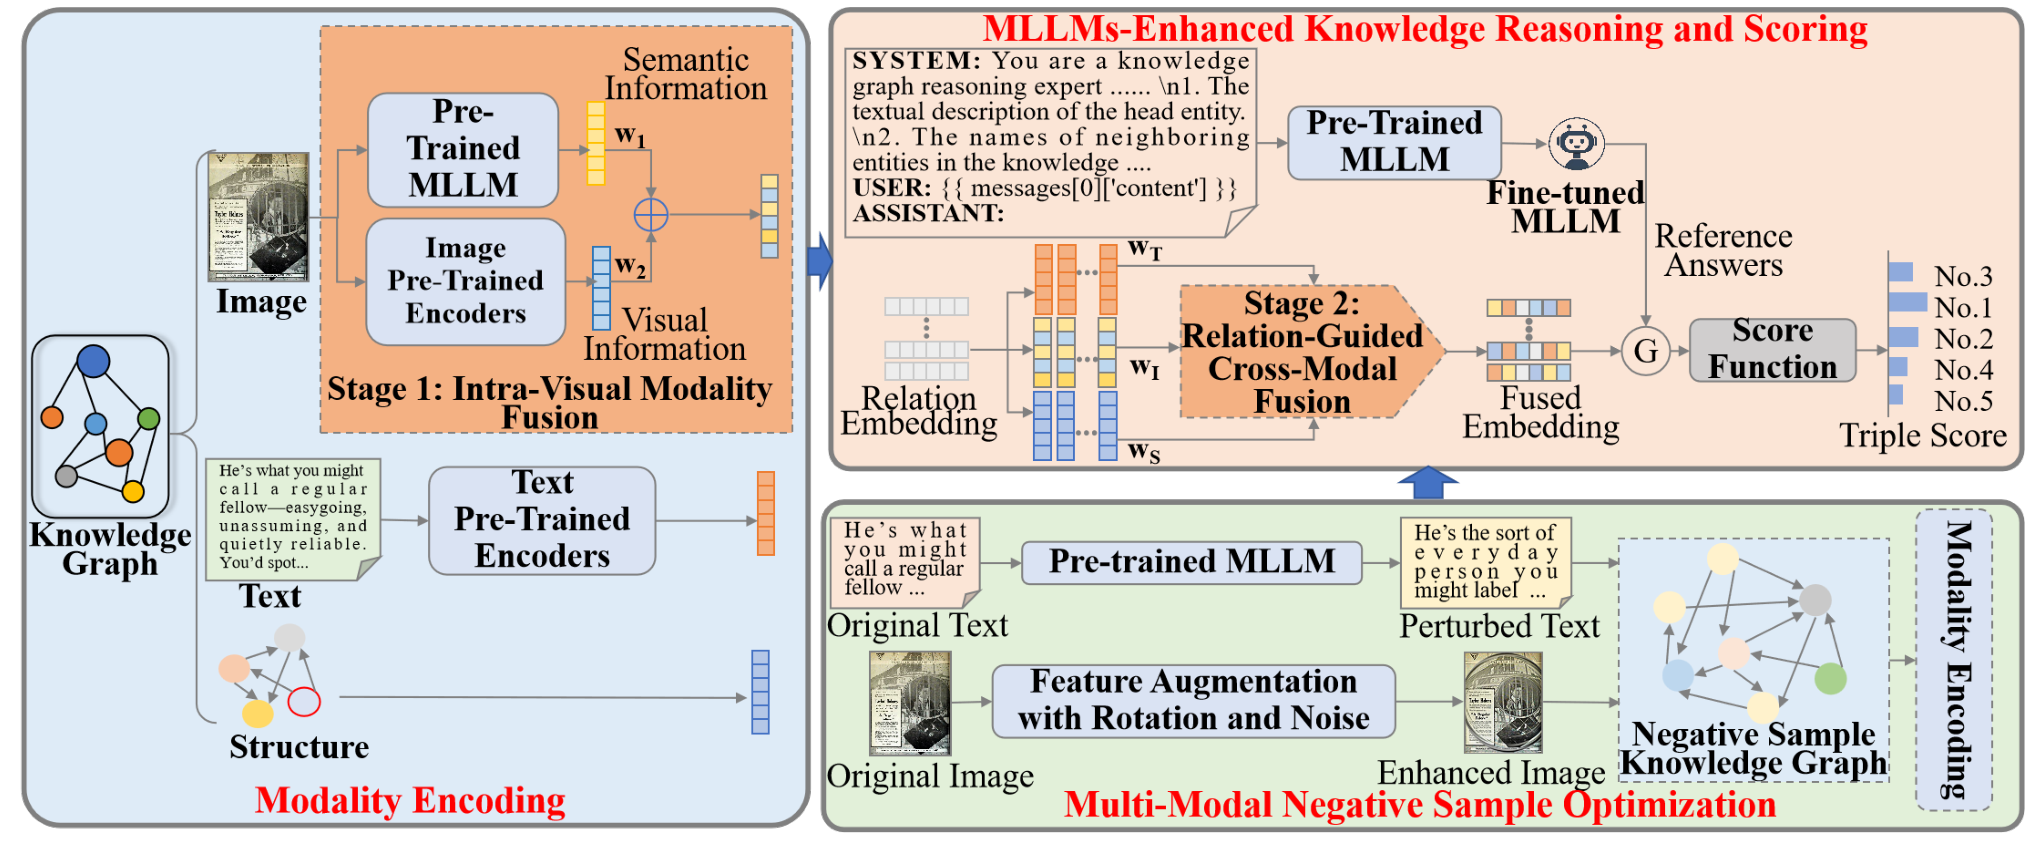
\includegraphics[width=0.92\textwidth]{hfr-fig2-architecture}
\caption{Kiến trúc HFR-MKGC theo hình gốc của tác giả (Hình 2 trong~\cite{hfrmkgc}). Bên trái: mã hoá ba mô thức và tầng 1 của RHF. Phải trên: tầng 2 của RHF, suy luận bằng MLLM và cổng $G$ trước hàm điểm. Phải dưới: sinh mẫu âm trong MNO.}
\label{fig:arch}
\end{figure*}

\begin{figure*}[t]
\centering
\begin{tikzpicture}[
  font=\small,
  box/.style={draw, rounded corners=2pt, minimum height=8mm, inner sep=3pt, align=center},
  inp/.style={box, minimum width=22mm},
  enc/.style={box, fill=gray!10, minimum width=30mm},
  fuse/.style={box, fill=cR!35},
  mllm/.style={box, fill=cG!25},
  score/.style={box, fill=black!80, text=white, minimum width=30mm, minimum height=12mm},
  arr/.style={-{Stealth[length=2.2mm]}, thick, cGray},
  lane/.style={draw, dashed, rounded corners=3pt, inner sep=4pt},
  lanelabel/.style={anchor=south west, font=\footnotesize\bfseries, inner sep=1pt}
]
% ===== Làn 1: thực thể đầu
\node[inp, fill=cI!20] (img) at (1.2, 0.0) {ảnh của $h$};
\node[inp, fill=cT!20] (txt) at (1.2,-1.75) {mô tả của $h$};
\node[inp, fill=cS!20] (id)  at (1.2,-2.85) {id của $h$};
\node[enc] (clip) at (4.6, 0.5)  {CLIP $\to P_I$};
\node[enc] (cap)  at (4.6,-0.55) {LLaVA viết caption\\$\to$ BERT $\to P_T$};
\node[enc] (bert) at (4.6,-1.75) {BERT $\to P_T$};
\node[enc] (tab)  at (4.6,-2.85) {tra bảng $\mathbf{E}$};
\node[fuse, minimum width=24mm] (s1) at (8.3, 0.0) {Tầng 1: gộp hai\\vector ảnh (sigmoid)};
\node[fuse, minimum width=24mm] (s2) at (11.4,-1.3) {Tầng 2: trộn $S,I,T$\\(softmax theo $r$)};
\node[box, fill=cR!60] (rel) at (11.4, 0.55) {vector quan hệ $r$};
\node[box, minimum width=14mm, minimum height=9mm] (hj) at (14.1,-1.3) {$\Hj$};
% ===== Làn 2: MER
\node[mllm] (prompt) at (1.85,-4.75) {prompt: mô tả, láng giềng,\\ảnh của $h$, tên quan hệ};
\node[mllm] (llava)  at (5.45,-4.75) {LLaVA-1.5-7B\\(LoRA)};
\node[mllm] (ans)    at (8.6,-4.75) {tên đáp án\\$\to$ BERT $\to \Tm$};
\node[mllm] (gate)   at (11.9,-4.75) {cổng $g$ = MLP\\hai lớp trên $\Tm$};
% ===== Làn 3: ứng viên đuôi
\node[box, dashed] (cand)  at (1.85,-6.85) {mỗi ứng viên $t$\\(toàn bộ $\sim$15k node)};
\node[fuse] (candrhf) at (5.45,-6.85) {Tầng 1 + 2 như trên\\(cùng $r$) $\to \Tj(t)$};
\node[box, fill=cG!25] (interp) at (11.9,-6.85) {$\Tt(t) = (1-g)\,\Tj(t)$\\$+\; g\,\Tm$};
% ===== Chấm điểm
\node[score] (rot)  at (16.2,-4.0) {RotatE: xoay $\Hj$\\theo $r$, đo khoảng\\cách tới $\Tt(t)$};
\node[box, minimum width=30mm] (rank) at (16.2,-6.85) {điểm $= -$khoảng cách\\$\to$ xếp hạng ứng viên};
% ===== Mũi tên làn 1
\draw[arr] (img.east) -- (clip.west);
\draw[arr] (img.east) -- (cap.west);
\draw[arr] (txt) -- (bert);
\draw[arr] (id) -- (tab);
\draw[arr] (clip.east) -- (s1.west);
\draw[arr] (cap.east) -- (s1.west);
\draw[arr] (s1.east) -- ($(s2.west)+(0,0.18)$);
\draw[arr] (bert.east) -- (s2.west);
\draw[arr] (tab.east) -- ($(s2.west)+(0,-0.18)$);
\draw[arr] (rel) -- (s2);
\draw[arr] (s2) -- (hj);
% ===== Mũi tên làn 2, 3
\draw[arr] (prompt) -- (llava);
\draw[arr] (llava) -- (ans);
\draw[arr] (ans) -- (gate);
\draw[arr] (gate) -- (interp);
\draw[arr] (ans.south) -- ++(0,-0.75) -| ($(interp.north west)+(0.45,0)$);
\draw[arr] (cand) -- (candrhf);
\draw[arr] (candrhf) -- (interp);
% ===== Vào RotatE
\draw[arr] (hj.east) -| ($(rot.north)+(-0.8,0)$);
\draw[arr] (rel.east) -| ($(rot.north)+(0.8,0)$);
\draw[arr] (interp.east) -- ++(0.55,0) |- (rot.west);
\draw[arr] (rot) -- (rank);
% ===== Khung làn
\begin{scope}[on background layer]
\node[lane, draw=cR!80!black, fit=(img)(id)(clip)(tab)(s1)(s2)(rel)(hj)] (L1) {};
\node[lane, draw=cG, fit=(prompt)(gate)] (L2) {};
\node[lane, draw=gray, fit=(cand)(interp)] (L3) {};
\end{scope}
\node[lanelabel, text=cR!60!black] at (L1.north west) {Mã hoá và RHF cho thực thể đầu $h$};
\node[lanelabel, text=cG] at (L2.north west) {MER: LLaVA đưa ra gợi ý};
\node[lanelabel, text=gray!70!black] at (L3.north west) {Chấm từng ứng viên đuôi};
\end{tikzpicture}
\caption{Luồng dữ liệu của một truy vấn $(h, r, ?)$ trong HFR-MKGC, nhóm vẽ lại từ mô tả trong~\cite{hfrmkgc}. Mỗi ứng viên đuôi đi qua cùng hàm RHF rồi được kéo về phía gợi ý của LLaVA theo tỉ lệ $g$; RotatE chỉ xoay thực thể đầu một lần và đo khoảng cách tới từng ứng viên. Khi huấn luyện, luồng này giữ nguyên và thêm nhánh MNO sinh mẫu âm (Mục~\ref{sec:hfr-mno}).}
\label{fig:pipeline}
\end{figure*}

\subsection{Biểu diễn thực thể và quan hệ}
\label{sec:hfr-encode}

Mỗi thực thể $e$ được lưu bằng \emph{ba} vector cùng chiều $d$, mỗi vector ứng với một mô thức $m \in \{S, I, T\}$:

\begin{itemize}
\item $\mathbf{e}_S$ (cấu trúc): một hàng trong bảng tham số $\mathbf{E} \in \mathbb{R}^{|\mathcal{E}| \times d}$, khởi tạo ngẫu nhiên, học từ đầu cùng toàn mô hình. Không có bước tiền huấn luyện riêng.
\item $\mathbf{e}_T$ (văn bản): đoạn mô tả qua BERT~\cite{bert} đóng băng, rồi qua một lớp chiếu học được $P_T$ để về chiều $d$.
\item $\mathbf{e}_I$ (ảnh): ảnh qua CLIP~\cite{clip} đóng băng rồi qua lớp chiếu $P_I$. Riêng mô thức này còn có một nhánh thứ hai mô tả ở Mục~\ref{sec:hfr-stage1}.
\end{itemize}

Quan hệ $r$ chỉ có \emph{một} vector $\mathbf{r} \in \mathbb{R}^d$, cũng khởi tạo ngẫu nhiên và học từ đầu; quan hệ không có ảnh hay văn bản. Vector này được dùng ở ba chỗ: làm ``câu hỏi'' khi tính trọng số trộn (Mục~\ref{sec:hfr-stage2}), làm góc xoay trong RotatE (Mục~\ref{sec:hfr-rotate}), và tên quan hệ dạng chữ được chèn vào prompt cho LLaVA (Mục~\ref{sec:hfr-mer}).

Vì CLIP và BERT xuất ra không gian khác nhau (512 và 768 chiều cho các bản thường dùng), hai lớp chiếu $P_I$, $P_T$ là chỗ duy nhất đưa chúng về cùng một không gian. Bài báo không có hàm mất mát căn chỉnh riêng cho việc này; hai lớp chiếu học gián tiếp qua hàm mất mát KGC cuối cùng. Nhóm quay lại điểm này ở Mục~\ref{sec:hfr-limits}.

\subsection{RHF tầng 1: gộp hai cách nhìn một tấm ảnh}
\label{sec:hfr-stage1}

Tầng 1 chỉ làm việc với ảnh, vì ảnh được mã hoá theo hai cách. Nhánh thị giác cho vector $\mathbf{e}_{I_v} = P_I(\mathrm{CLIP}(\text{ảnh}))$. Nhánh ngữ nghĩa cho LLaVA~\cite{llava} viết một câu mô tả ảnh (caption, ví dụ ``a woman singing on stage''), rồi câu đó qua BERT và $P_T$ thành $\mathbf{e}_{I_c}$. Hai vector nói về cùng một tấm ảnh nhưng ở hai dạng: một dạng là đặc trưng thị giác thô, một dạng đã được dịch sang ngôn ngữ, gần với thế giới của KG hơn.

Cách gộp là một cổng không có tham số:
\begin{equation}
\sigma = \mathrm{sigmoid}\big(\langle \mathbf{e}_{I_v}, \mathbf{e}_{I_c}\rangle\big), \qquad
\mathbf{e}_I = \sigma\,\mathbf{e}_{I_c} + (1-\sigma)\,\mathbf{e}_{I_v}.
\label{eq:stage1}
\end{equation}
Tích vô hướng đo hai cách nhìn có khớp nhau không. Khớp cao thì $\sigma$ gần 1, tin caption nhiều hơn; khớp thấp nghĩa là caption có thể tả sai, giữ đặc trưng CLIP. Quy ước ``caption nhận $\sigma$, CLIP nhận $1-\sigma$'' là do tác giả cố định; nếu đảo lại mô hình vẫn học được vì không có tham số nào gắn với quy ước đó, nhưng ý đồ ``khi hai bên đồng ý thì ưu tiên dạng ngôn ngữ'' là lý do chọn chiều này.

Cần nhấn mạnh: tầng này không học gì. Tham số học nằm ở $P_I$ và $P_T$; chúng phải tự xoay hai không gian sao cho tích vô hướng ở~\eqref{eq:stage1} có nghĩa, và động lực duy nhất để làm vậy là hàm mất mát KGC ở cuối.

\subsection{RHF tầng 2: trộn ba mô thức theo quan hệ}
\label{sec:hfr-stage2}

Đây là mô-đun quan trọng nhất và cũng là chữ ``relation-guided'' trong tên bài. Cho thực thể $e$ với ba vector $\mathbf{e}_S, \mathbf{e}_I, \mathbf{e}_T$ và quan hệ $\mathbf{r}$, mỗi mô thức $m$ nhận một điểm thô:
\begin{equation}
\alpha_m = \underbrace{\langle \mathbf{e}_m, \mathbf{r}\rangle}_{\text{liên quan tới câu hỏi}}
 + \underbrace{\frac{1}{3}\sum_{j \in \{S,I,T\}} \langle \mathbf{e}_m, \mathbf{e}_j\rangle}_{\text{nhất quán với hai mô thức kia}}.
\label{eq:alpha}
\end{equation}
Số hạng thứ nhất là chỗ làm trọng số đổi theo quan hệ: cùng $\mathbf{e}_I$ nhưng tích với vector của voice type khác tích với vector của place of birth. Số hạng thứ hai lấy trung bình độ tương đồng với các mô thức của chính thực thể (gồm cả với chính nó), để hạ điểm những mô thức lạc lõng, ví dụ ảnh mặc định do thiếu dữ liệu hoặc mô tả bị bịa.

Ba điểm thô qua softmax thành ba tỉ lệ cộng bằng 1, rồi pha ba vector theo tỉ lệ đó:
\begin{equation}
w_m = \frac{\exp(\alpha_m)}{\sum_j \exp(\alpha_j)}, \qquad
\Hj = \sum_{m} w_m\,\mathbf{e}_m .
\label{eq:hjoint}
\end{equation}
Softmax ở đây chạy trên \emph{ba con số}, không phải trên ba vector; mỗi mô thức nhận đúng một trọng số dùng chung cho mọi chiều.

\paragraph{Ví dụ chạy tay.}
Để thấy cơ chế, nhóm chọn $d = 3$ với các số tự đặt (không phải số của bài báo):
$\mathbf{e}_S = [0{,}5;\,0{,}1;\,-0{,}3]$,
$\mathbf{e}_I = [0{,}8;\,0{,}7;\,0{,}1]$,
$\mathbf{e}_T = [-0{,}1;\,0{,}9;\,0{,}6]$,
$\mathbf{r} = [-0{,}2;\,1{,}0;\,0{,}5]$.
Số hạng thứ nhất của~\eqref{eq:alpha} cho $-0{,}15$, $0{,}59$, $1{,}22$; số hạng thứ hai cho $0{,}22$, $0{,}73$, $0{,}55$. Cộng lại $\alpha = [0{,}07;\,1{,}32;\,1{,}77]$, softmax cho $w = [0{,}10;\,0{,}35;\,0{,}55]$ và $\Hj = [0{,}275;\,0{,}750;\,0{,}335]$. Nếu bỏ số hạng chứa $\mathbf{r}$, trọng số thành $[0{,}24;\,0{,}41;\,0{,}35]$: ảnh lên cao nhất, văn bản rớt xuống. Hình~\ref{fig:weights} vẽ hai bộ trọng số này. Đó chính là khác biệt giữa HFR-MKGC và các mô hình trộn không nhìn quan hệ: cùng một thực thể, đổi câu hỏi thì tỉ lệ đổi theo, nhưng số tham số không tăng vì cái được lưu vẫn chỉ là ba vector.

\begin{figure}[t]
\centering
\begin{tikzpicture}
\begin{axis}[
  ybar, bar width=9pt, width=\linewidth, height=4.2cm,
  ymin=0, ymax=0.7, ylabel={trọng số $w_m$},
  symbolic x coords={S,I,T}, xtick=data, xticklabels={cấu trúc $S$, ảnh $I$, văn bản $T$},
  enlarge x limits=0.3,
  legend style={at={(0.5,1.02)}, anchor=south, legend columns=2, font=\footnotesize, draw=none},
  tick label style={font=\footnotesize}, label style={font=\footnotesize},
  nodes near coords, nodes near coords style={font=\scriptsize},
  every node near coord/.append style={/pgf/number format/.cd, fixed, precision=2}
]
\addplot[fill=cR!70, draw=cR!60!black] coordinates {(S,0.10) (I,0.35) (T,0.55)};
\addplot[fill=gray!40, draw=gray] coordinates {(S,0.24) (I,0.41) (T,0.35)};
\legend{{có số hạng $\langle \mathbf{e}_m{,} \mathbf{r}\rangle$},{không có (như trộn cố định)}}
\end{axis}
\end{tikzpicture}
\caption{Trọng số trộn ở tầng 2 trong ví dụ chạy tay ($d=3$, số liệu nhóm tự đặt để minh hoạ). Có vector quan hệ, văn bản thắng; bỏ đi, ảnh thắng. Hình do nhóm vẽ.}
\label{fig:weights}
\end{figure}

Về bản chất,~\eqref{eq:alpha}--\eqref{eq:hjoint} là một phép chú ý (attention) rút gọn: truy vấn là chính $\mathbf{r}$, khoá và giá trị là chính các vector mô thức, không có ma trận chiếu $W_Q, W_K, W_V$. Cách thiết kế này giữ tầng 2 không có tham số, giống tầng 1.

\subsection{MER: cho LLaVA gợi ý, nhưng không cho nó chấm điểm}
\label{sec:hfr-mer}

Mô-đun MER đưa mô hình ngôn ngữ lớn đa phương thức LLaVA-1.5-7B vào vòng lặp theo bốn bước.

\textbf{Bước 1, hỏi.} Với mỗi truy vấn $(h, r, ?)$, ghép một prompt gồm phần hướng dẫn cố định, đoạn mô tả của $h$, tên các láng giềng của $h$ trong đồ thị, ảnh của $h$ và tên quan hệ $r$ dạng chữ. LLaVA được tinh chỉnh bằng LoRA~\cite{lora} cho đúng nhiệm vụ này; phần nối CLIP với mô hình ngôn ngữ bên trong LLaVA là có sẵn từ dự án LLaVA, tác giả chỉ thêm các ma trận hạng thấp. Đầu ra là \emph{một chuỗi tên}, ví dụ ``Mezzo-soprano''.

\textbf{Bước 2, mã hoá.} Chuỗi đó qua BERT và lớp chiếu thành vector $\Tm \in \mathbb{R}^{2d}$ (chiều $2d$ vì hàm điểm RotatE làm việc với $d$ số phức, xem Mục~\ref{sec:hfr-rotate}). Mỗi truy vấn chỉ tính $\Tm$ một lần.

\textbf{Bước 3, cổng.} Một mạng hai lớp đọc $\Tm$ và xuất ra mức tin cậy theo từng chiều:
\begin{equation}
\mathbf{g} = \mathrm{sigmoid}\big(W_2\,\tanh(W_1 \Tm + \mathbf{b}_1) + \mathbf{b}_2\big) \in (0,1)^{2d},
\label{eq:gate}
\end{equation}
với $W_1 \in \mathbb{R}^{d \times 2d}$, $W_2 \in \mathbb{R}^{2d \times d}$. Đây là chỗ \emph{có} tham số học, khác hai cổng không tham số ở RHF.

\textbf{Bước 4, kéo ứng viên về phía gợi ý.} Với mỗi ứng viên đuôi $t$, trước hết tính $\Tj(t)$ bằng đúng hàm RHF hai tầng ở trên (cùng vector $\mathbf{r}$), rồi pha với gợi ý theo từng chiều:
\begin{equation}
\Tt(t) = (\mathbf{1} - \mathbf{g}) \odot \Tj(t) + \mathbf{g} \odot \Tm .
\label{eq:interp}
\end{equation}
Mọi ứng viên bị dịch một đoạn về phía $\Tm$; ứng viên nào vốn đã gần gợi ý thì sau khi dịch càng gần điểm neo của RotatE. Nếu $\mathbf{g}$ gần 0, mô hình bỏ qua LLaVA và quay về RotatE thuần. Thực thể đầu không bị kéo; bài báo có nhắc tới $\tilde{\mathbf{H}}_{\mathrm{joint}}$ nhưng không định nghĩa, nên nhóm hiểu là thực thể đầu dùng thẳng $\Hj$.

Điểm nhóm thấy đáng bàn: $\mathbf{g}$ chỉ nhìn $\Tm$, không nhìn $\Hj$ hay $\mathbf{r}$. Cổng do đó học ``đáp án kiểu này đáng tin bao nhiêu'' chứ không học ``đáp án này có hợp với câu hỏi này không''. Nếu LLaVA trả về một tên có thật nhưng sai quan hệ, cổng khó phát hiện.

\subsection{Hàm điểm RotatE}
\label{sec:hfr-rotate}

HFR-MKGC không đề xuất hàm điểm mới mà dùng RotatE~\cite{rotate}, chỉ thay đầu vào bằng các vector đã trộn. Trong RotatE, mỗi thực thể là một vector $d$ số phức, lưu bằng $2d$ số thực (nửa đầu phần thực, nửa sau phần ảo), tức $d$ điểm trên $d$ mặt phẳng độc lập. Quan hệ là $d$ góc xoay $\theta_k$, lấy từ vector $\mathbf{r}$ bằng cách chia cho một hằng số $\gamma$ và nhân $\pi$, rồi đổi thành số phức mô-đun 1:
\begin{equation}
\theta_k = \pi\,\frac{r_k}{\gamma}, \qquad r^{\mathbb{C}}_k = \cos\theta_k + i\sin\theta_k .
\end{equation}
Điểm của một bộ ba là âm khoảng cách giữa thực thể đầu sau khi xoay và thực thể đuôi:
\begin{equation}
f(h, r, t) = -\big\lVert \Hj \circ \mathbf{r}^{\mathbb{C}} - \Tt(t) \big\rVert ,
\label{eq:score}
\end{equation}
trong đó $\circ$ là nhân từng phần tử trên số phức, tức xoay điểm thứ $k$ một góc $\theta_k$ trên mặt phẳng thứ $k$ (Hình~\ref{fig:rotate}). Trên số thực, phép xoay là $a' = a\cos\theta - b\sin\theta$, $b' = a\sin\theta + b\cos\theta$, nên cài đặt không cần kiểu dữ liệu phức.

\begin{figure}[t]
\centering
\begin{tikzpicture}[scale=1.15, font=\footnotesize]
\draw[->, gray] (-1.6,0) -- (1.9,0) node[below] {Re};
\draw[->, gray] (0,-0.4) -- (0,2.1) node[left] {Im};
\coordinate (h) at (1.5,0.35);
\coordinate (hr) at ({1.5*cos(55)-0.35*sin(55)},{1.5*sin(55)+0.35*cos(55)});
\coordinate (t1) at (0.62,1.42);
\coordinate (t2) at (-0.9,0.9);
\draw[cS, thick, -{Stealth}] (0,0) -- (h) node[right] {$\Hj$ (Gwen)};
\draw[cR!70!black, thick, dashed, -{Stealth}] (0.9,0.21) arc[start angle=13, end angle=68, radius=0.92] node[midway, above right, xshift=1pt] {$\theta$ (voice type)};
\draw[cR!70!black, thick, -{Stealth}] (0,0) -- (hr) node[above right, xshift=-6pt, yshift=1pt] {$\Hj \circ r^{\mathbb{C}}$ (điểm neo)};
\fill[cT] (t1) circle (1.6pt) node[right, xshift=2pt, cT!60!black] {$\Tt$(Mezzo-soprano)};
\fill[cI] (t2) circle (1.6pt) node[left, cI!70!black] {$\Tt$(Double bass)};
\draw[cT!60!black, thick, dotted] (hr) -- (t1) node[midway, below right, xshift=-2pt, yshift=-1pt] {gần};
\draw[cI!70!black, thick, dotted] (hr) -- (t2) node[midway, above, yshift=1pt] {xa};
\end{tikzpicture}
\caption{RotatE trên một trong $d$ mặt phẳng phức: xoay thực thể đầu theo góc của quan hệ rồi đo khoảng cách tới từng ứng viên. Xoay chỉ làm một lần cho mỗi truy vấn; đo lặp lại cho mọi ứng viên. Hình do nhóm vẽ, minh hoạ ý tưởng, không theo số liệu thật.}
\label{fig:rotate}
\end{figure}

Lý do giữ RotatE: một phép xoay mô tả được ba kiểu quan hệ thường gặp. Quan hệ đối xứng ứng với góc $180^\circ$ (xoay hai lần trở về chỗ cũ), quan hệ nghịch đảo ứng với góc đối $-\theta$, và quan hệ hợp thành ứng với cộng góc $\theta_1 + \theta_2$. Việc biểu diễn trong không gian phức không phải điểm mới của bài; nó kế thừa từ ComplEx~\cite{complex} và RotatE. Đóng góp của HFR-MKGC nằm ở \emph{thứ được đưa vào} hàm điểm: $\Hj$ đã trộn theo $r$ và $\Tt$ đã được LLaVA kéo.

Tổng kết luồng suy diễn cho (Gwen Stefani, voice type, ?): mã hoá ba mô thức của Gwen, trộn theo quan hệ voice type ra $\Hj$, xoay theo $d$ góc của voice type ra điểm neo; song song, LLaVA trả lời ``Mezzo-soprano'', mã hoá thành $\Tm$ và tính $\mathbf{g}$; với từng ứng viên trong 15000 thực thể, tính $\Tj$ rồi $\Tt$, đo khoảng cách tới điểm neo, xếp hạng. Không có ngưỡng ``có cạnh hay không''; kết quả là một thứ hạng. Đáp án của LLaVA chỉ dịch chuyển các ứng viên, không bao giờ là đáp án cuối.

\subsection{MNO: mẫu âm khó và huấn luyện đối kháng}
\label{sec:hfr-mno}

Huấn luyện KGE cần mẫu âm. Cách thường dùng là thay $t$ bằng một thực thể ngẫu nhiên; mẫu như vậy quá dễ phân biệt nên tín hiệu học yếu dần. MNO giữ nguyên thực thể và bóp méo đặc trưng của nó theo hai cách:

\begin{itemize}
\item \textbf{Văn bản:} LLaVA viết lại đoạn mô tả theo cách khác (paraphrase), rồi mã hoá bằng BERT như thường.
\item \textbf{Ảnh:} vector CLIP $\mathbf{x}$ được xoay và cộng nhiễu:
\begin{equation}
\hat{\mathbf{x}} = \big((1-\lambda)\mathbf{I} + \lambda\mathbf{R}\big)\mathbf{x} + \boldsymbol{\epsilon}, \quad \boldsymbol{\epsilon} \sim \mathcal{N}(0, \sigma^2 \mathbf{I}),
\label{eq:perturb}
\end{equation}
với $\mathbf{R}$ là ma trận trực giao lấy từ phân rã QR của một ma trận hạng thấp, và $\lambda$ tăng tuyến tính theo epoch: đầu khoá học mẫu giả gần bản gốc, cuối khoá học lệch xa hơn (curriculum).
\end{itemize}

Từ một bộ ba đúng $(h, r, t)$ sinh ba bộ giả $(h^*, r, t)$, $(h, r, t^*)$, $(h^*, r, t^*)$, trong đó dấu sao là bản bị bóp méo. Chúng được chấm bằng cùng hàm điểm~\eqref{eq:score}.

Phần huấn luyện là một trò chơi hai bên (Hình~\ref{fig:mno}). Bên ``phân biệt'' là chính mô hình KGC, tối thiểu hoá
\begin{equation}
\mathcal{L}_D = \mathcal{L}_{\mathrm{kgc}} + \mu_1\,\mathcal{L}_{\mathrm{gp}},
\label{eq:ld}
\end{equation}
trong đó $\mathcal{L}_{\mathrm{kgc}}$ là hàm mất mát tự đối kháng của RotatE (mẫu âm khó hơn nhận trọng số softmax lớn hơn) tính trên cả mẫu âm thường và mẫu giả, còn $\mathcal{L}_{\mathrm{gp}}$ là phạt gradient kiểu WGAN-GP~\cite{wgangp} để ổn định. Bên ``sinh'' là bộ bóp méo, tối thiểu hoá
\begin{equation}
\mathcal{L}_G = \sum_{k} \max\big(0,\; c - f(\text{bộ giả}_k)\big),
\label{eq:lg}
\end{equation}
tức bị phạt khi mẫu giả bị nhận ra quá dễ (điểm thấp hơn ngưỡng $c$). Hai bên cập nhật xen kẽ. Khung đối kháng này kế thừa từ AdaMF-MAT~\cite{adamf}; phần mới của bài là cách sinh mẫu giả bằng LLM và ma trận xoay.

\begin{figure}[t]
\centering
\begin{tikzpicture}[font=\footnotesize, node distance=4mm and 6mm,
  box/.style={draw, rounded corners=2pt, align=center, inner sep=2.5pt, minimum height=7mm, text width=29mm},
  arr/.style={-{Stealth[length=2mm]}, thick, cGray}]
\node[box, fill=cT!20] (pos) {bộ ba đúng $(h,r,t)$\\+ mẫu âm thường (thay $t$ ngẫu nhiên)};
\node[box, fill=cG!25, right=5mm of pos] (gen) {Bộ sinh $G$: paraphrase văn bản (LLaVA), xoay + nhiễu ảnh~\eqref{eq:perturb}};
\node[box, fill=gray!10, below=of gen] (fake) {bộ giả $(h^*,r,t)$, $(h,r,t^*)$, $(h^*,r,t^*)$};
\node[box, fill=black!80, text=white, below=of pos, yshift=-11mm, text width=66mm] (dis) {Bộ phân biệt $D$ = chính mô hình KGC (RHF + MER + RotatE), chấm điểm mọi bộ ba bằng~\eqref{eq:score}};
\node[box, fill=cR!35, below=of dis.south west, anchor=north west] (ld) {$\mathcal{L}_D$~\eqref{eq:ld}: điểm thật cao, điểm giả và âm thấp, + phạt gradient};
\node[box, fill=cR!35, below=of dis.south east, anchor=north east] (lg) {$\mathcal{L}_G$~\eqref{eq:lg}: phạt $G$ khi điểm giả thấp hơn ngưỡng $c$};
\draw[arr] (pos.south) -- (pos.south |- dis.north);
\draw[arr] (gen) -- (fake);
\draw[arr] (fake.south) -- (fake.south |- dis.north);
\draw[arr] (dis.south -| ld.north) -- (ld.north);
\draw[arr] (dis.south -| lg.north) -- (lg.north);
\draw[arr, dashed, cG] (lg.east) -- ++(3mm,0) |- (gen.east);
\draw[arr, dashed] (ld.west) -- ++(-3mm,0) |- (dis.west);
\end{tikzpicture}
\caption{Vòng huấn luyện đối kháng của MNO. Bộ phân biệt chính là mô hình KGC; hai hàm mất mát được tối ưu xen kẽ. Mũi tên đứt nét tím: cập nhật bộ sinh $G$; đứt nét xám: cập nhật $D$. Hình do nhóm vẽ.}
\label{fig:mno}
\end{figure}

Nhận xét của nhóm: một đoạn văn ``cùng nghĩa, khác lời'' và một ảnh xoay nhẹ về bản chất vẫn là thực thể gốc. Bài coi chúng là bộ ba sai nhưng không kiểm chứng điều đó. Cách hiểu hợp lý hơn là hàm mất mát chỉ ép điểm của bản gốc cao hơn bản giả một chút, làm ranh giới quanh mỗi thực thể sắc hơn, thay vì thật sự dạy mô hình phân biệt đúng và sai. Đây cũng là chỗ MDBGF đi theo giả định ngược lại (Phần~\ref{sec:mdbgf}).

\subsection{Những gì được học và không được học}

Để tiện đối chiếu, Bảng~\ref{tab:params} liệt kê tham số học và tham số đóng băng. Điều đáng chú ý là hai cổng của RHF đều không có tham số; toàn bộ sức ``thích nghi theo quan hệ'' đến từ việc bảng $\mathbf{E}$, bảng $\mathbf{R}$ và hai lớp chiếu cùng học qua một hàm mất mát duy nhất.

\begin{table}[t]
\centering
\caption{Thành phần học được và đóng băng trong HFR-MKGC (nhóm tổng hợp từ~\cite{hfrmkgc}).}
\label{tab:params}
\footnotesize
\begin{tabular}{l l}
\toprule
Thành phần & Trạng thái\\
\midrule
Bảng thực thể $\mathbf{E}$, bảng quan hệ $\mathbf{R}$ & học từ đầu\\
Lớp chiếu $P_I$, $P_T$ & học\\
Cổng $\mathbf{g}$ (MLP hai lớp) & học\\
LoRA trong LLaVA (nhiệm vụ đoán đáp án) & học\\
Cổng tầng 1, softmax tầng 2 & không có tham số\\
CLIP, BERT, phần còn lại của LLaVA & đóng băng\\
\bottomrule
\end{tabular}
\end{table}

\subsection{Thực nghiệm}
\label{sec:hfr-exp}

\paragraph{Thiết lập.} Tác giả huấn luyện 250 epoch bằng Adam trên hai GPU RTX A6000, chọn chiều $d \in \{128, 256, 512\}$, số mẫu âm mỗi bộ ba trong $\{32, 64, 128\}$, tốc độ học trong $\{10^{-5}, 10^{-4}, 10^{-3}\}$ và kích thước batch trong $\{128, 256, 1024\}$. Vì nhiều mô hình cơ sở không công khai đủ mã hay dữ liệu, tác giả tự chạy lại chúng với cùng bộ mã hoá CLIP và BERT. Nhóm \emph{không} tái lập được HFR-MKGC vì mã nguồn không công khai, nên mọi số liệu dưới đây là của bài báo.

\paragraph{Kết quả chính.} Bảng~\ref{tab:main} rút gọn từ Bảng 1 của bài, giữ RotatE làm mốc, các mô hình MMKGC mạnh nhất và LLaVA chạy đơn độc. Ba quan sát:

\begin{enumerate}
\item So với mô hình cơ sở tốt nhất NativE, HFR-MKGC tăng MRR 1{,}83 điểm trên MKG-W và 1{,}61 điểm trên DB15K nhưng chỉ 0{,}66 điểm trên MKG-Y. MKG-Y có 28 quan hệ, cấu trúc đã đủ mạnh nên đa mô thức thêm được ít; điều này nhất quán với động lực của bài.
\item HFR-MKGC đứng đầu 11 trong 12 ô. Ngoại lệ là Hits@1 trên DB15K (23{,}04\%), thua RSME, APKGC và MyGO. Bài viết rằng phương pháp đạt mức tốt nhất trên mọi độ đo; nhóm cho rằng cần nói chính xác là 11/12.
\item LLaVA dùng một mình kém xa mọi mô hình KGE, đặc biệt trên MKG-Y (Hits@10 bằng 3{,}58\%). LLM không thay được hàm điểm có cấu trúc; vai trò hợp lý của nó là bổ trợ, đúng như cách MER thiết kế.
\end{enumerate}

\begin{table*}[t]
\centering
\caption{Kết quả chính (\%), rút gọn từ Bảng 1 của~\cite{hfrmkgc}. Tốt nhất in đậm, tốt thứ hai gạch chân (tính trên toàn bộ 14 mô hình cơ sở của bài, không chỉ các dòng hiển thị). LLaVA không tính được MRR vì chỉ sinh 10 ứng viên.}
\label{tab:main}
\footnotesize
\setlength{\tabcolsep}{4.5pt}
\begin{tabular}{l cccc cccc cccc}
\toprule
\multirow{2}{*}{Mô hình} & \multicolumn{4}{c}{MKG-W} & \multicolumn{4}{c}{MKG-Y} & \multicolumn{4}{c}{DB15K}\\
\cmidrule(lr){2-5}\cmidrule(lr){6-9}\cmidrule(lr){10-13}
 & MRR & H@10 & H@3 & H@1 & MRR & H@10 & H@3 & H@1 & MRR & H@10 & H@3 & H@1\\
\midrule
RotatE~\cite{rotate}   & 32.92 & 44.23 & 35.91 & 26.68 & 36.67 & 41.11 & 35.91 & 33.92 & 32.07 & 51.40 & 38.57 & 21.23 \\
RSME~\cite{rsme}       & 33.41 & 44.31 & 35.80 & 27.59 & 38.03 & 44.02 & 35.80 & \underline{34.28} & \underline{33.72} & 50.39 & 39.23 & \textbf{24.45} \\
MyGO~\cite{mygo}       & 33.40 & 44.36 & 35.38 & 27.52 & 30.29 & 42.17 & 35.38 & 23.75 & 32.25 & 48.23 & 35.49 & 24.19 \\
AdaMF-MAT~\cite{adamf} & 32.09 & 45.78 & 35.54 & 24.48 & 37.78 & 46.11 & 35.54 & 32.65 & 32.08 & 52.42 & 40.41 & 19.81 \\
APKGC~\cite{apkgc}     & 32.67 & 46.20 & 35.83 & 25.24 & 31.48 & 40.68 & 35.83 & 26.17 & 32.91 & 48.91 & 37.15 & \underline{24.39} \\
NativE~\cite{native}   & \underline{36.79} & \underline{50.28} & \underline{40.47} & \underline{29.36} & \underline{38.34} & \underline{46.24} & \underline{40.47} & 33.49 & 33.59 & \underline{53.77} & \underline{40.67} & 22.11 \\
LLaVA~\cite{llava} (chỉ suy diễn) & --- & 26.42 & 22.29 & 15.02 & --- & 03.58 & 02.80 & 01.64 & --- & 15.89 & 13.15 & 08.32 \\
\midrule
HFR-MKGC~\cite{hfrmkgc} & \textbf{38.62} & \textbf{51.66} & \textbf{42.12} & \textbf{31.37} & \textbf{39.00} & \textbf{47.31} & \textbf{42.12} & \textbf{34.41} & \textbf{35.20} & \textbf{56.41} & \textbf{43.25} & 23.04 \\
\bottomrule
\end{tabular}
\end{table*}

\paragraph{Loại bỏ từng phần.} Bảng~\ref{tab:ablation} là nghiên cứu loại bỏ, chỉ làm trên MKG-W. Nhóm đọc bảng này theo hai hướng.

Theo mô-đun: bỏ RHF (thay bằng trung bình cộng ba mô thức) mất nhiều nhất, 6{,}64 điểm MRR. Đáng chú ý là Hits@10 gần như không đổi (50{,}25 so với 51{,}66) trong khi Hits@1 rớt từ 31{,}37 xuống 20{,}80. Nghĩa là trộn theo quan hệ không giúp tìm thêm ứng viên vào top 10, mà giúp \emph{xếp đúng ứng viên lên hạng nhất}. Bỏ MER mất 5{,}10 điểm, bỏ MNO mất 4{,}61 điểm; thay cách bóp méo của MNO bằng nhiễu ngẫu nhiên (w/o PTI) mất 4{,}03 điểm, cho thấy cách sinh mẫu giả có ý nghĩa chứ không chỉ là thêm nhiễu.

Theo mô thức: bỏ cấu trúc mất 12{,}95 điểm, vẫn là mô thức quan trọng nhất; bỏ văn bản mất nhiều hơn bỏ ảnh (8{,}95 so với 7{,}46); bỏ riêng caption do LLaVA sinh (w/o VT) mất 6{,}84 điểm, chứng tỏ tầng 1 của RHF có ích thật.

\begin{table}[t]
\centering
\caption{Loại bỏ từng phần trên MKG-W (\%), theo Bảng 3 của~\cite{hfrmkgc}. Cột cuối do nhóm tính.}
\label{tab:ablation}
\footnotesize
\setlength{\tabcolsep}{4pt}
\begin{tabular}{l cccc r}
\toprule
Thiết lập & MRR & H@10 & H@3 & H@1 & $\Delta$MRR\\
\midrule
w/o S (bỏ cấu trúc)           & 25.67 & 39.42 & 28.81 & 18.02 & $-12{,}95$\\
w/o T (bỏ văn bản)            & 29.67 & 45.61 & 34.92 & 21.25 & $-8{,}95$\\
w/o V (bỏ ảnh)                & 31.16 & 47.39 & 36.10 & 22.09 & $-7{,}46$\\
w/o VT (bỏ caption ảnh)       & 31.78 & 47.33 & 36.41 & 23.22 & $-6{,}84$\\
\midrule
w/o RHF (trộn trung bình)     & 31.98 & 50.25 & 39.14 & 20.80 & $-6{,}64$\\
w/o MER (bỏ LLaVA gợi ý)      & 33.52 & 50.61 & 39.70 & 23.42 & $-5{,}10$\\
w/o PTI (nhiễu ngẫu nhiên)    & 34.59 & 50.95 & 40.03 & 25.12 & $-4{,}03$\\
w/o MNO (bỏ đối kháng)        & 34.01 & 50.98 & 40.26 & 24.13 & $-4{,}61$\\
\midrule
HFR-MKGC đầy đủ               & \textbf{38.62} & \textbf{51.66} & \textbf{42.12} & \textbf{31.37} & ---\\
\bottomrule
\end{tabular}
\end{table}

\paragraph{Độ nhạy siêu tham số.} Tác giả quét chiều $d$ và số mẫu âm trên MKG-W cho cả HFR-MKGC và RotatE. Kết luận có thể dùng được: chiều lớn (512) chỉ phát huy khi có nhiều mẫu âm (128); chiều 256 tốt nhất với 64 mẫu âm; chiều 128 gần như không nhạy với số mẫu âm. MRR và Hits@1 dao động mạnh hơn Hits@10, nhất quán với nhận xét ở phần loại bỏ rằng các mô-đun chủ yếu tác động lên thứ hạng đầu.

\paragraph{Nghiên cứu tình huống.} Hình~\ref{fig:case} là ví dụ của tác giả với đúng truy vấn Gwen Stefani. Khi thay RHF bằng trọng số ngẫu nhiên, ảnh nhận trọng số cao nhất dù chỉ chứa ngoại hình, và Mezzo-soprano đứng hạng 2. Với RHF, trọng số văn bản tăng, ảnh giảm, đáp án đúng lên hạng 1. Đây là minh chứng định tính cho cơ chế ở Mục~\ref{sec:hfr-stage2}.

\begin{figure}[t]
\centering
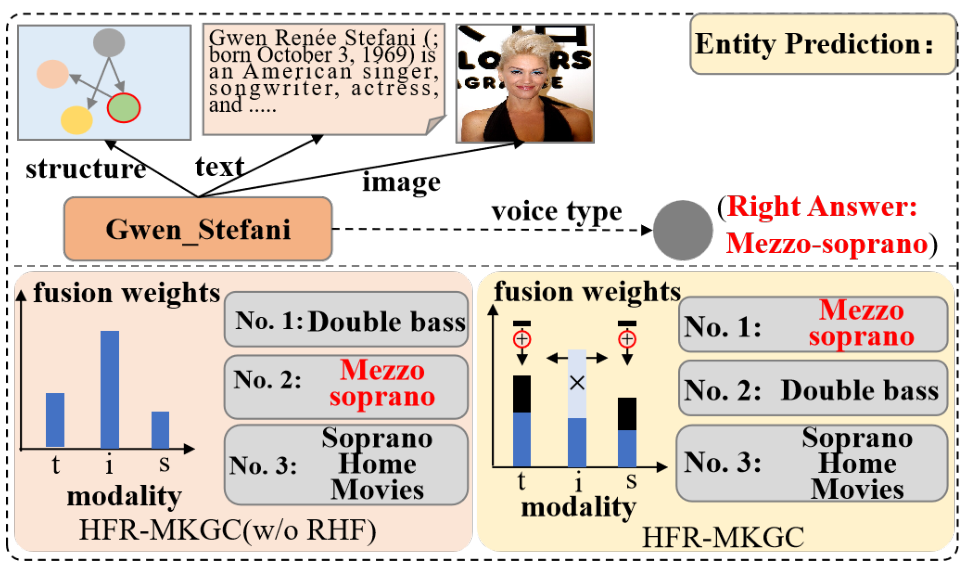
\includegraphics[width=\linewidth]{hfr-fig4-case-study}
\caption{Nghiên cứu tình huống của tác giả (Hình 4 trong~\cite{hfrmkgc}): trọng số mô thức và thứ hạng ứng viên cho (Gwen Stefani, voice type, ?) khi không có và có RHF.}
\label{fig:case}
\end{figure}

\subsection{Nhận xét và hạn chế}
\label{sec:hfr-limits}

Nhóm tổng hợp các điểm chưa thuyết phục, chia thành ba nhóm.

\textbf{Về phương pháp.}
(1) Việc so CLIP với BERT bằng tích vô hướng ở~\eqref{eq:stage1} và~\eqref{eq:alpha} chỉ có nghĩa nếu hai lớp chiếu đã đưa chúng về cùng không gian, nhưng bài không có hàm mất mát căn chỉnh riêng và không nói có chuẩn hoá vector hay không. Mọi căn chỉnh đều gián tiếp qua hàm mất mát KGC.
(2) Cổng $\mathbf{g}$ không nhìn ngữ cảnh câu hỏi (Mục~\ref{sec:hfr-mer}).
(3) Mẫu giả trong MNO không được kiểm chứng là sai thật (Mục~\ref{sec:hfr-mno}).
(4) Nhiều siêu tham số không được nêu: nội dung prompt, số epoch tinh chỉnh LoRA, cách chọn láng giềng đưa vào prompt, các hằng $\gamma$, $c$, $\mu_1$, nhiệt độ của hàm mất mát tự đối kháng, tỉ lệ bước cập nhật $D$ và $G$.

\textbf{Về thực nghiệm.}
(5) Cải thiện không đều: MKG-Y chỉ tăng 0{,}66 MRR; thua Hits@1 trên DB15K; tuyên bố ``tốt nhất trên mọi độ đo'' là quá mức.
(6) Loại bỏ từng phần chỉ làm trên một bộ dữ liệu.
(7) Chi phí không được báo cáo: LLaVA-7B phải chạy cho mỗi ảnh (caption), mỗi truy vấn (gợi ý) và mỗi đoạn văn bản (paraphrase), nhưng bài không nêu thời gian huấn luyện hay suy diễn so với mô hình cơ sở.
(8) Không công khai mã nguồn, và nhiều mô hình cơ sở do tác giả tự chạy lại, nên khó kiểm chứng độc lập.

\textbf{Về rò rỉ tri thức.} (9) LLaVA và BERT được tiền huấn luyện trên dữ liệu web có thể đã ``biết'' các sự thật trong Wikidata hay DBpedia. Bài không thảo luận khả năng này, dù nó ảnh hưởng trực tiếp tới cách diễn giải đóng góp của MER.

Dù vậy, ý tưởng cốt lõi của bài, theo nhóm, là đúng hướng và đơn giản: trọng số trộn mô thức phải phụ thuộc câu hỏi đang hỏi, và LLM nên là người gợi ý chứ không phải người chấm điểm. Hai ý này không phụ thuộc vào RotatE và có thể ghép vào hàm điểm khác.

% =====================================================================
\section{Phần B: MDBGF}
\label{sec:mdbgf}

\todo{Phần này sẽ viết sau khi nhóm đọc xong bài báo. Khung dự kiến dưới đây.}

\subsection{Động lực và ý tưởng chính}
\todo{Vấn đề mô thức thiếu/nhiễu trong thực tế; vì sao ``không phải mọi mô thức cùng lúc''.}

\subsection{Dynamic Dropout}
\todo{Cách rụng mô thức khi huấn luyện, lịch rụng, khác dropout thường thế nào.}

\subsection{Bidirectional Fusion}
\todo{Hai chiều hợp nhất là gì, công thức, vai trò của contrastive loss.}

\subsection{Thực nghiệm}
\todo{Kết quả trên MKG-W, MKG-Y, DB15K; thiết lập thiếu mô thức; loại bỏ từng phần. Nếu nhóm chạy lại bằng mã nguồn tác giả, gắn link WandB công khai và link repo GitHub tại đây.}

\subsection{Nhận xét và hạn chế}
\todo{}

% =====================================================================
\section{Đối chiếu hai bài và kết luận}
\label{sec:compare}

\todo{Hoàn thiện sau khi xong Phần B.} Điểm đối chiếu nhóm đã thấy từ phía HFR-MKGC: hai bài cùng dùng ba bộ dữ liệu, cùng đặt câu hỏi ``dùng ảnh và văn bản thế nào cho bền vững'', nhưng chọn hai giả định ngược nhau về các biến thể của một thực thể. HFR-MKGC coi bản bóp méo là mẫu âm cần đẩy xa; MDBGF (theo nhóm hiểu sơ bộ) coi các mô thức của cùng thực thể là thứ cần kéo gần nhau và dùng dropout để mô hình quen với việc thiếu. HFR-MKGC căn chỉnh mô thức gián tiếp qua hàm mất mát KGC; MDBGF căn chỉnh tường minh. HFR-MKGC đưa LLM vào vòng lặp với chi phí lớn; MDBGF không dùng LLM.

\bibliographystyle{IEEEtran}
\bibliography{references}

\end{document}
